
% Include LaTeX packages
\documentclass[conference]{styles/acmsiggraph}
\usepackage{comment} % enables the use of multi-line comments (\ifx \fi)
\usepackage{fullpage}
\usepackage{enumitem}
\usepackage{amsmath,amsthm,amssymb}
\usepackage{listings}
\usepackage{graphicx}
\usepackage{etoolbox}
\usepackage{verbatim}
\usepackage{minted}
\usepackage[dvipsnames]{xcolor}
\usepackage{fancyvrb}
\usepackage{hyperref}
\usepackage{menukeys}
\usepackage{titlesec}
\usepackage{csquotes}
\usepackage{placeins}
\usepackage{caption}
\usepackage{subcaption}
\usepackage{algorithm} 
\usepackage{booktabs}
\usepackage{cases} 
\usepackage{algpseudocode}
\usepackage{unicode-math}
\newcommand{\?}{\stackrel{?}{=}}
\renewcommand\qedsymbol{$\blacksquare$}
\usepackage{tikz}


\usepackage[T1]{fontenc}
\usepackage{kantlipsum}
\usepackage[usenames,dvipsnames]{xcolor}
\usepackage[breakable, theorems, skins]{tcolorbox}
\tcbset{enhanced}

\DeclareRobustCommand{\myalignbox}[2][gray!20]{%
\begin{tcolorbox}[   %% Adjust the following parameters at will.
        breakable,
        left=0pt,
        right=0pt,
        top=0pt,
        bottom=12pt,
        colback=#1,
        colframe=#1,
        width=\dimexpr\textwidth\relax, 
        enlarge left by=0mm,
        boxsep=5pt,
        arc=0pt,outer arc=0pt,
        ]
        #2
\end{tcolorbox}
}

\DeclareRobustCommand{\myTIKZbox}[2][gray!20]{%
\begin{tcolorbox}[   %% Adjust the following parameters at will.
        breakable,
        left=0pt,
        right=0pt,
        top=10pt,
        bottom=12pt,
        colback=#1,
        colframe=#1,
        width=\dimexpr\textwidth\relax, 
        enlarge left by=0mm,
        boxsep=5pt,
        arc=0pt,outer arc=0pt,
        ]
        #2
\end{tcolorbox}
}

\DeclareRobustCommand{\mybox}[2][gray!20]{%
\begin{tcolorbox}[   %% Adjust the following parameters at will.
        breakable,
        left=0pt,
        right=0pt,
        top=0pt,
        bottom=0pt,
        colback=#1,
        colframe=#1,
        width=\dimexpr\textwidth\relax, 
        enlarge left by=0mm,
        boxsep=5pt,
        arc=0pt,outer arc=0pt,
        ]
        #2
\end{tcolorbox}
}

% Set additional LaTeX options
\setlength{\parskip}{.8mm}
\setcounter{MaxMatrixCols}{20}
\hypersetup{
	colorlinks=true,
	urlcolor=[rgb]{0.97,0,0.30},
	anchorcolor={0.97,0,0.30},
	linkcolor=black,
	filecolor=[rgb]{0.97,0,0.30},
}

% Define title, author, and affiliation information
\title{\huge PSET 7 \\ \LARGE {CS124: Data Structures and Algorithms \\ Prof. Mitzenmacher}}
\author{\Large Dhilan Ramaprasad \\ dhilanramaprasad@college.harvard.edu}
\pdfauthor{Student Name}

% Redefine \VerbatimInput
\RecustomVerbatimCommand{\VerbatimInput}{VerbatimInput}%
{fontsize=\footnotesize,
 %
 frame=lines, % top and bottom rule only
 framesep=2em, % separation between frame and text
 rulecolor=\color{Gray},
 %
 label=\fbox{\color{Black}\textbf{OUTPUT}},
 labelposition=topline,
 %
 commandchars=\|\(\), % escape character and argument delimiters for commands within the verbatim
 commentchar=* % comment character
}

% Set addditional formatting options
\titlespacing*{\section}{0pt}{5.5ex plus 1ex minus .2ex}{2ex}
\titlespacing*{\subsection}{0pt}{3ex}{2ex}
\setcounter{secnumdepth}{4}
\renewcommand\theparagraph{\thesubsubsection.\arabic{paragraph}}
\newcommand\subsubsubsection{\paragraph}

% Define a convenient norm symbol
\newcommand{\norm}[1]{\left\lVert#1\right\rVert}
\renewcommand{\vec}[1]{\mathbf{#1}}

% Define a macro for hiding answers
\newbool{hideanswers} \setbool{hideanswers}{false}
\newenvironment{answer}{}{}
\ifbool{hideanswers}{\AtBeginEnvironment{answer}{\comment} %
\AtEndEnvironment{answer}{\endcomment}}{}

% Define text formatting for points and normals
\newcommand{\points}[1]{\hfill \normalfont{(\textit{#1pts})}}
\newcommand{\pointsin}[1]{\normalfont{(\textit{#1pts})}}







%%%%%%%%%%%%%%%%%%%%%%%%%%%%%%%%%%%%%%%
%%%%%%%%%%%%%%%%%%%%%%%%%%%%%%%%%%%%%%%
%%%%%%%%%%%%%%%%%%%%%%%%%%%%%%%%%%%%%%%
%%%%%%%%%%%%%%%%%%%%%%%%%%%%%%%%%%%%%%%
%%%%%%%%%%%%%%%%%%%%%%%%%%%%%%%%%%%%%%%

         %  START HERE  %

%%%%%%%%%%%%%%%%%%%%%%%%%%%%%%%%%%%%%%%
%%%%%%%%%%%%%%%%%%%%%%%%%%%%%%%%%%%%%%%
%%%%%%%%%%%%%%%%%%%%%%%%%%%%%%%%%%%%%%%
%%%%%%%%%%%%%%%%%%%%%%%%%%%%%%%%%%%%%%%
%%%%%%%%%%%%%%%%%%%%%%%%%%%%%%%%%%%%%%%

\begin{document}
\maketitle

\textbf{Collaborator}: No one :( \\
\textbf{Others:} Advice from Phil, Benny, Marwa, and Jaylen (throughout CS124). \\
\\
As an Electrical Engineering concentrator, I've made a great effort to avoid theoretical CS thoughout my short academic career (seeing as I chose the major sophomore fall).  Slowness of my code implementations never scared me; after all, the solution was simple: make better transistors, improve micro-architectures, add stream buffers, more caches, lessen the cost of SRAM, introduce out-of-order processors, parallelize.  The closest I ever came to an algorithm was Belady's algorithm for cache member eviction, or Tomosulo's algorithm which has nothing to do with algorithms, or that one time 'Lil Yachty said \enquote{you Harvard kids like algorithms, right} during Yard Fest 2018. \\

But the times have changed.  In passing, I asked Eddie K., \enquote{Hey, should I switch to a joint with CS?}  And he swiftly replied, \enquote{YES!}  And so a new dilemma arose: (1) \textbf{take CS124 junior spring \textit{or}} (2) \textbf{take CS20 now} and CS124 \textit{senior spring}.  The latter, of course, was not an option; after all, I wouldn't know anyone in the course :(  \\

So I sucked it up, concurrently enrolled in a statistics class (ES150, sadly not STAT110), cried my way through the first PSET with a trip to Mitz's office hours for help on the hardest mathematical proof we did all semester, followed by a late Gradescope submission as I wasted precious hours of PSET2 time to get my matrix multiplication to work (my \verb|Cpp| skills were crusty despite being fresh out of CS61). \\

Here's what I realized: \textbf{CS124 is doable.}  It's not as horrifying as people make it out to be.  And yes, I have submitted each of my PSETs $\geq$ 1 day late after going remote, but if I were on campus, I would have finished in time with no problem because I would have had the greatest team known to man by my side throughout these latter 3 PSETs.\\

Just like the crew of Apollo 13, when it came to \textbf{Benny Paris} (OSB, as the world knows him, the master of storytelling in Overleaf and in person, half the brains and all the wit of our operation), \textbf{Phil Nicol} (ask him about tumor generator or all things Cpp---oh, also, he's the other half of the brains and the \textit{entirety} of the looks of our operation), and \textbf{Dhilan} (not much to contribute---no brains, no looks---but above average \verb|.tex| formatting and the occasional mediocre code snippet)---failure was not an option---we were unstoppable. \\

Now, while I will never have the opportunity for Mitz to hand me a failing grade (unless I successfully cop an unsat or \textit{UEM}), I can rest easy knowing that even if I failed, I succeeded in being member to one of the most iconic teams in human history.  Thank you to Benny and Phil for everything.  Thank you to Rajath for nothing.  Thank you to Esther and Amy for your early guidance.  Thank you to Rachel and Rose for great sections.  And of course, the biggest, uh, like, thank you to an inspiration: \textbf{Mitz.}

\newpage




%%%%%%%%%%%%%%%%%%%%%%%%%%%%%%%%%%%%%%%
%%%%%%%%%%%%%%%%%%%%%%%%%%%%%%%%%%%%%%%
%%%%%%%%%%%%%%%%%%%%%%%%%%%%%%%%%%%%%%%
%%%%%%%%%%%%%%%%%%%%%%%%%%%%%%%%%%%%%%%
%%%%%%%%%%%%%%%%%%%%%%%%%%%%%%%%%%%%%%%

        %  PROBLEMS HERE  %

%%%%%%%%%%%%%%%%%%%%%%%%%%%%%%%%%%%%%%%
%%%%%%%%%%%%%%%%%%%%%%%%%%%%%%%%%%%%%%%
%%%%%%%%%%%%%%%%%%%%%%%%%%%%%%%%%%%%%%%
%%%%%%%%%%%%%%%%%%%%%%%%%%%%%%%%%%%%%%%
%%%%%%%%%%%%%%%%%%%%%%%%%%%%%%%%%%%%%%%




\section{Go with the Flow}
%%%%%%%%%%%%%%%%%%
%   Question #1  %
%%%%%%%%%%%%%%%%%%
\textbf{Setup:} We are given the maximum flow (value and flow along each edge) in a graph $G = (V,E)$ with source $s$, sink $t$, and integer capacities.

\subsection{Increased by 1}
Given that the capacity of one edge in our graph is increased by $1$, we can easily find a linear time algorithm to compute the new maximum flow.\\

\mybox{
We first need to construct the residual graph given the original maximum flow for the unchanged (no incremented edge capacity) graph.  It can be assumed that this can be done in O(|V|+|E|) time as we have the information for flow across each edge a priori. \\

Now, on the residual graph, we can add in our change: the increased capacity to an edge.  Running Ford-Fulkerson, we run DFS in O(|V| + |E|), but seeing as we know that the max-flow has increased by \textbf{at most} 1, we only need to run DFS once to find the augmenting path (i.e., path from $s$ to $t$ along which we can increase flow, specifically by $1$ in this case) if it exists.  Naturally, if the path exists, increase the flow, add $1$ to our prior maximum flow, and return the new residual graph.}\\

It is worth noting explicitly that the maximum flow is an integer value (due to integer capacities) and it increases at most by 1.  This comes naturally from our discussion in lecture and section of finding an min S-T cut which demonstrates the maximum flow of G.  Of course, now one capacity may have increased by $1$ along this cut, but no more than that, so the maximum flow may only increase by 1.  Note that it cannot decrease.

\subsection{Decreased by 1}
The decrementing scenario requires two cases (quite non-trivial).  Initially, I thought we could use the residual graph again and find a path from $t$ to $s$ this time, but I am not so sure that works.\\

\mybox{
Instead, consider the first case where the selected edge $(u,v) \in E$ for decreased capacity $c'(e) = c(e) - 1$ had flow (given in the original graph) which was less than its original capacity---i.e., $f(e) < c(e)$:  \textbf{then, there is no change to the maximum flow} as there was \enquote{over-capacity} at the start (before decrementing).\\

In the case where original $f(e) = c(e)$ for the selected edge, $e$, then we must determine whether another augmenting path can compensate for the lost flow.  The process is as follows: \textbf{(1)} construct the residual graph, \textbf{(2)} find a path from $s$ to $t$ containing the selected edge, $e$, and reduce flow on each edge in the found path such that now the flow to $t$ has dropped by $1$, \textbf{(3)} now seek a new augmenting path (if one exists) from $s$ to $t$ by running Ford-Fulkerson with DFS once (knowing that our max-flow can at most return to what it was prior---the original value---but cannot change further given it was \textit{max} prior to our decremented capacity), \textbf{(4)} if a new augmenting path is found, we can increase flow along the path and note the new flow along edges traversed and note that the max flow value is unchanged as there was more than one unique solution to the max flow problem on the original graph; else, if no new path is found, return our adjusted graph with decremented edges, and return the new inflow to $t$ as our updated max flow (which is just decremented by 1).\\

The \textbf{runtime} is O(|V| + |E|) to make the residual graph, O(|V| + |E|) to find a path from $s$ to $t$ containing the selected edge (via BFS), and O(|V| + |E|) for one run of Ford-Fulkerson $\implies$ O(|V| + |E|).}

\newpage


\section{The War for Independence}
%%%%%%%%%%%%%%%%%%
%   Question #2  %
%%%%%%%%%%%%%%%%%%
\subsection{Line on $n$ vertices}
First let's explore a few values and scenario: if we define the function $I(n)$ to return the number of independent sets given $n$-node line, taking the empty set to be an independent set $\implies$ when $n=0$, $I(0) = 1$.  See Table \ref{tab:line} for more selected values:

% Table generated by Excel2LaTeX from sheet 'Sheet1'
\begin{table}[htbp]
  \centering
    \begin{tabular}{c|c}
    \multicolumn{1}{c}{n} & I(n) \\
    \midrule
    0     & 1 \\
    1     & 2 \\
    2     & 3 \\
    3     & 5 \\
    4     & 8 \\
    \end{tabular}%
    \caption{Number of Independent Sets, varied size-$n$ of line graph}
  \label{tab:line}%
\end{table}%
\FloatBarrier

\mybox{
By observation, $\mathbf{I(n)}$ returns $\mathbf{I(n-2) + I(n-1)}$.  This recurrence, given its starting value (base case) $I(0) = 1$, can be represented by the requested \enquote{family of numbers} which are the \textbf{Fibonacci} numbers.  Specifically, $I(n) = \text{Fib}(n+2)$
}\\

\textbf{Note:} My definition of \textit{Fibonacci} numbers follows that of \verb|mathworld.wolfram.com| wherein $\text{Fib}(1) = \text{Fib}(2) = 1$.\\

The proof of the recurrence comes in that adjacent nodes cannot both be in the independent set (as the set would no longer be independent), so we can isolate our $n$th case as follows:
\begin{enumerate}
    \item Take node $n$ to \textbf{not} be part of the independent set.  Then node $n-1$ (being adjacent) surely \textit{can} be member to many independent sets without node $n$, and its representation is simply $I(n-1)$.
    \item Now take node $n$ to be member to the independent set.  Because in the prior step we have counted all eligible steps up to $n-1$ nodes where node $n-1$ may or may not be in the independent set, we must be careful not to double count sets.  It is naive to say if node $n$ is now an eligible member, node $n-1$ is no longer an active member, so we can take $I(n-1)$ again, as that would over-count.  So we can imagine now restricting ourselves to all of the independent sets wherein node $n$ \textbf{must} be member.  This is represented by $I(n-2)$ which represents all of the independent sets wherein (1) node $n-1$ is not member and (2) node $n$ is not member; however, given we've already accounted for all scenarios of (2), we can take $I(n-2)$ to actually represent all of the independent sets wherein (1) node $n-1$ is not member and now (2) node $n$ is \textbf{member to all} thereby ensuring these $I(n-2)$ sets are unique---not double counts---and thereby exhaustively covering all constructible independent sets.
\end{enumerate}

\newpage
\subsection{Cycle on $n$ vertices}
First let's explore a few values and scenario: if we define the function $K(n)$ to return the number of independent sets given $n$-node cycle, taking the empty set to be an independent set $\implies$ when $n=0$, $K(0) = 1$.  See Table \ref{tab:cycle} for more selected values:

\begin{table}[htbp]
  \centering
    \begin{tabular}{c|c}
    \multicolumn{1}{c}{n} & K(n) \\
    \midrule
    0     & 1 \\
    1     & 2 \\
    2     & 3 \\
    3     & 4 \\
    4     & 7 \\
    5     & 11 \\
    6     & 18 \\
    \end{tabular}%
    \caption{Number of Independent Sets, varied size-$n$ of cycle graph}
    \label{tab:cycle}
\end{table}%
\FloatBarrier

\mybox{
After $n = 3$ (the first \enquote{standard} cycle), we can see a simple recurrence wherein $\mathbf{K(n) = K(n-1) + K(n-2)}$ which neatly matches the same recurrence as the Fibonacci numbers, but its base cases differ, so the recurrence for $n > 3$ actually maps to the family entitled \textbf{Lucas numbers}.
$$\text{for Lucas numbers, }L_1 = 1\text{ and }L_2 = 3\text{, and }L_n = L_{n-1} + L_{n-2}\text{ [just like Fibonacci]}$$

In the proceeding analysis, it just so happens that $\mathbf{K(n) = I(n-1) + I(n-3)}$ for all $n$ using our prior recurrence for line graphs.
}



The proof of the recurrence again comes in that adjacent nodes cannot both be in the independent set (as the set would no longer be independent), so we can isolate our $n$th case \textbf{and reduce to the prior scenario (line graph)} as follows:
\begin{enumerate}
    \item Take node $n$ to \textbf{not} be part of the independent set.  Then node $n-1$ and node $0$ (being adjacent left and adjacent right, respectively) surely \textit{can} be member to many independent sets without node $n$, and so our representation of all the number of independent sets sans node $n$ is simply $I(n-1)$ as we have one fewer node which can be represented as being extracted from the graph leaving a line graph of size $n-1$.
    \item Now take node $n$ to be member to the independent set.  Because in the prior step we have counted all eligible steps up to $n-1$ nodes where nodes $0$ and $n-1$ may or may not be in the independent set, we must be careful not to double count sets.  We can imagine now restricting ourselves to all of the independent sets wherein node $n$ \textbf{must} be member.  This is represented by $I(n-3)$ which represents a line graph of size $n-3$ (i.e., missing nodes $0$, $n-1$, and $n$) which would seem to double count cases, but we now consider that node $n$ is \textbf{member to all} of these $I(n-3)$ counted sets which makes them unique from those counted previously, exhaustively covering all constructible independent sets.
\end{enumerate}

\newpage
\subsection{Complete binary tree}
Let us begin by notating a few convenient factors and terms.  First, for a complete binary tree, the number of nodes is one minus power of 2---i.e., $n = 2^k - 1$ where $k$ conveniently represents the \enquote{height} or depth of the tree (number of 
\enquote{levels}).\\

Like our prior similar question regarding \textit{set cover} with binary trees, we know that there are two scenarios: (1) take root and grandchildren (optional in the case of constructing any independent sets---unlike in set cover) but \textbf{not} children, and (2) take children but \textbf{not} root or grandchildren.\\

Naturally, we see that the number of children is 2 to every parent, and the number of grandchildren is 4 to every grandparent (original root).  If the parent is at level $k$ with. $2^k - 1$ nodes, each child is a sub-tree composed of $2^{k-1} - 1$ nodes, and each grandchild now roots a sub-tree composed of $2^{k-2} - 1$ nodes.\\

Let's take $\mathbf{T(k)}$ to represent the number of independent sets given by a complete binary tree of height $k$ where we have the base cases $T(0) = 1$ and $T(1) = 2$.\\

Suppose \textbf{we now examine the root of a tree of height $k$:}\\using the multiplication rule in independent probability/counting (from statistics), we know that for children of the first node there are $T(k-1) \times T(k-1)$ independent set options (given there are \textbf{2} children each of whom are roots to a sub-tree of height $k-1$).\\

Similarly, for grandchildren, $\exists\  T(k-2) \times T(k-2) \times T(k-2) \times T(k-2) $ independent set options (given there are \textbf{4} grandchildren each of whom are roots to a sub-tree of height $k-2$).

Let's now follow a similar strategy as before (line and circle graphs) wherein we \textbf{take \textit{or} exclude} the root (node $n$) and have a two-term sum recurrence.  The term of the recurrence which represents inclusion of the root \textit{is} counting correctly because, like before, it mandates inclusion of the root (node $n$) in \textbf{all} independent sets counted by the term, which prohibits any double counting---i.e., counted sets are unique.\\

We will sum the cases where (1) we include the root (and thereby grandchildren are eligible, though not required) which prohibits any children being included, and (2) the case where we do \textbf{not} include the root, thereby, we are left with the children subtrees and are free to create independent sets on the smaller trees whose total count will multiply as stated before:

$$\implies T(k) = \underbrace{T(k-1) \times T(k-1)}_{\text{children}} + \underbrace{T(k-2) \times T(k-2) \times T(k-2) \times T(k-2)}_{\text{grandchildren}}$$



\mybox{
From the Online Encyclopedia of Integer Sequences (OEIS), the result could be found, but a Python script was used to confirm: for $127$ nodes ($k = 7$), the number of independent sets is $\mathbf{13345346031444632841427643906}$}


\newpage

\textbf{Code Exerpt:}\\
\begin{minted}{python}
def T(n):
    if n == 0:
      return 1
    elif n == 1:
      return 2
    else:
      return T(n-1)*T(n-1) + T(n-2)*T(n-2)*T(n-2)*T(n-2)
\end{minted}


\newpage


\section{MAX-$k$-CUT}
%%%%%%%%%%%%%%%%%%
%   Question #3  %
%%%%%%%%%%%%%%%%%%
\subsection{Randomized Algorithm}
Taking our randomized algorithm for MAX CUT, the generalization here, is simple.  Suppose we have a $k$-sided die.  Roll the die to place each vertex into a set numbered $(1,2,\ldots, k)$.\\

The probability a vertex, $v \in V$, is in set $k$ is naturally $P(v \in S_k) = \frac{1}{k}$.  For a given edge, $(u,v) \in E$, the probability it crosses between sets (any two distinct sets) is the probability that $u$ and $v$ are not in the same set:

$$ P((u,v) \in E \text{ crosses between sets}) = P(v \notin S_k \mid u \in S_k) = 1 - P(v \in S_k \mid u \in S_k)$$
$$\implies P((u,v) \in E \text{ crosses between sets}) =  1 - \frac{1}{k}$$

\mybox{
Given the above, we now find the expectation (i.e., the expected number of edges crossing between sets):
$$\mathbf{E[}(u,v)\text{ crosses between sets } \forall (u,v) \in E\mathbf{]} = |E| \cdot \left (1 - \frac{1}{k}\right)$$

The upper bound on edges crossing any of $k$-cuts is O(|E|), so our randomized algorithm has an approximation factor of $\left (1 - \frac{1}{k}\right)$.
}


\subsection{Local Search}
We can begin to approach the algorithm as we did in lecture:

\mybox{
\textbf{WHILE $\exists$} a vertex $(v \in V)$ that increases the MAX-$k$-CUT by moving to a new disjoint set $k$, move the vertex $v$.}

\textbf{First, we should show termination of this algorithm:}\\
We know that there is an upper bound on the cut size (as seen when examining the randomized algorithm), so at some point, there will definitively \textbf{not} be a moveable vertex which will increase the MAX-$k$-CUT beyond its intrinsic limit.\\

\textbf{Now, let's examine the division of a vertex and its neighbors given termination of the algorithm:}\\
Just as in lecture, we can bound the number of neighbors a vertex has in each set---i.e., for each vertex, no more than $\frac{1}{k}$ of its neighbors are in its final assigned set; else, we'd move the vertex to a new set such that we could capitalize on an increase in number of edges crossing the cuts.  In other words, where $\delta(v)$ represents the neighbors of a vertex, $v$, we know that $\left (1 - \frac{1}{k}\right) \cdot \delta(v)$ connecting vertices are in other sets $\implies \geq \left (1 - \frac{1}{k}\right) \cdot \delta(v)$ edges crossing between sets per vertex.\\

\textbf{Finally, let's perform some \textit{adapted} accounting to prove performance bound:}
\begin{enumerate}
    \item Take any vertex $v \in S_i$
    \item For every vertex $w \in S_{j}, j \neq i$, add $\frac{1}{2}$ to a running sum.
    \item Repeat for each vertex in each set---i.e. $\forall v \in S_{i}, i = \{1,2, \ldots,k\}$
\end{enumerate}

In mathematical notation, where $C$ is the number of crossing edges:
\begin{equation}
    C = \frac{1}{2} \left(  \sum_{v \in S_1}  \left | \{w\text{: } (v,w) \in E, w \in S_{j}, j \neq 1\} \right | + \cdots +  \sum_{v \in S_k}  \left | \{w\text{: } (v,w) \in E, w \in S_{j}, j \neq k\} \right | \right)
\end{equation}

Knowing a lower bound for the edges crossing between sets per vertex as delineated above to be 1 - $\frac{1}{k}$.  We can rewrite $C$ as follows:
\begin{align}
    C \geq \frac{1}{2} \left(  \sum_{v \in S_1}  \left(1 - \frac{1}{k}\right) \delta(v) + \cdots +  \sum_{v \in S_k}  \left(1 - \frac{1}{k}\right) \delta(v) \right) \\
    C \geq \left(\frac{1}{2}\right) \left(1 - \frac{1}{k}\right)\left(  \sum_{v \in S_1}\delta(v) + \cdots +  \sum_{v \in S_k} \delta(v) \right) \\
    C \geq \left(\frac{1}{2}\right) \left(1 - \frac{1}{k}\right)\underbrace{\sum_{v \in V}\delta(v)}_{\leq 2|E|}\\
    \implies C \geq \left(\frac{1}{2}\right) \left(1 - \frac{1}{k}\right) 2|E|
\end{align}

\mybox{
We have shown, then that the number of crossing edges is bounded below by $C \geq \left(1 - \frac{1}{k}\right) |E|$.  The upper bound on edges crossing any of $k$-cuts is O(|E|), so our randomized algorithm has an approximation factor of $\left (1 - \frac{1}{k}\right)$.
}

\newpage


\section{It never really \textit{clique'd}}
%%%%%%%%%%%%%%%%%%
%   Question #4  %
%%%%%%%%%%%%%%%%%%
I'd like to preface this solution with an apology.  I spent too much time on the other problems, leaving this for last, and naturally, my solution demonstrates what the kids often call \textit{a weak showing.}  I would say, \enquote{I will do better next time,} but seeing as this is the last pset---well, uh, like---I'm sorry.  Nevertheless, I hope some of what I have said merits partial credit :)

\subsection{Examples and clique size in $\mathbf{G'}$:}
Let's explore two simple examples:

%% TIKZ PICS    
\begin{center}
    \tikzset{every picture/.style={line width=0.75pt}} %set default line width to 0.75pt        
    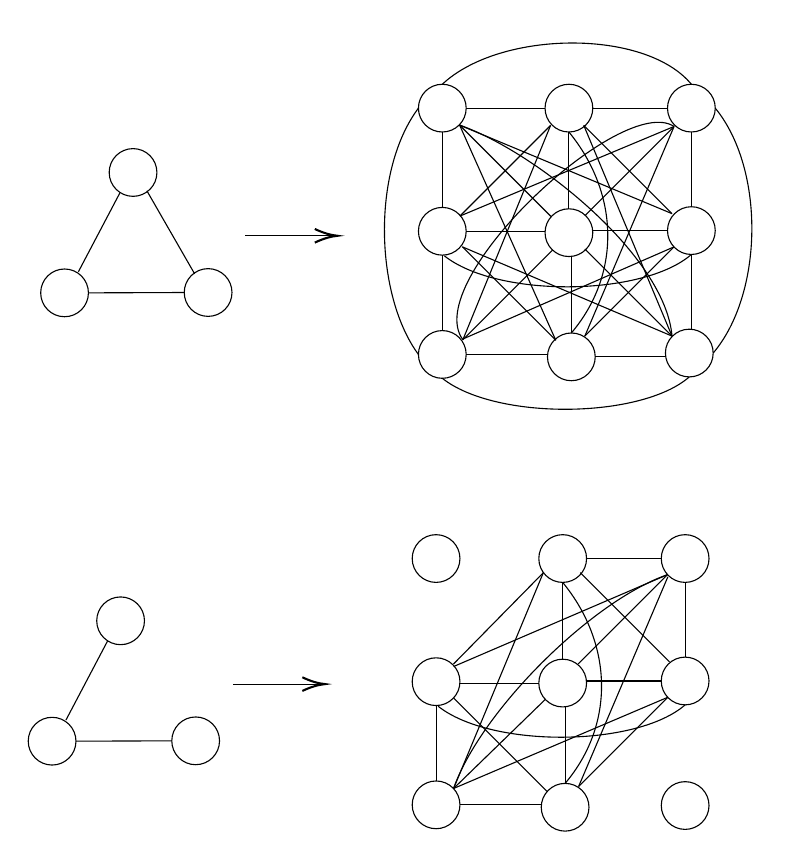
\begin{tikzpicture}[x=0.75pt,y=0.75pt,yscale=-1,xscale=1]
    %uncomment if require: \path (0,442); %set diagram left start at 0, and has height of 442
    
    %Shape: Circle [id:dp2354998254867846] 
    \draw   (203,70.5) .. controls (203,64.15) and (208.15,59) .. (214.5,59) .. controls (220.85,59) and (226,64.15) .. (226,70.5) .. controls (226,76.85) and (220.85,82) .. (214.5,82) .. controls (208.15,82) and (203,76.85) .. (203,70.5) -- cycle ;
    %Shape: Circle [id:dp0003468264981381086] 
    \draw   (170,128.5) .. controls (170,122.15) and (175.15,117) .. (181.5,117) .. controls (187.85,117) and (193,122.15) .. (193,128.5) .. controls (193,134.85) and (187.85,140) .. (181.5,140) .. controls (175.15,140) and (170,134.85) .. (170,128.5) -- cycle ;
    %Shape: Circle [id:dp4134071778258759] 
    \draw   (239.17,128.33) .. controls (239.17,121.98) and (244.32,116.83) .. (250.67,116.83) .. controls (257.02,116.83) and (262.17,121.98) .. (262.17,128.33) .. controls (262.17,134.68) and (257.02,139.83) .. (250.67,139.83) .. controls (244.32,139.83) and (239.17,134.68) .. (239.17,128.33) -- cycle ;
    %Straight Lines [id:da03322506525937774] 
    \draw    (208.17,80.33) -- (188.17,118.33) ;
    %Straight Lines [id:da10829630530082368] 
    \draw    (221.17,79.33) -- (244.17,119.33) ;
    %Straight Lines [id:da09584382201131803] 
    \draw    (193,128.5) -- (239.17,128.33) ;
    %Shape: Circle [id:dp4951446020026069] 
    \draw   (352,39.5) .. controls (352,33.15) and (357.15,28) .. (363.5,28) .. controls (369.85,28) and (375,33.15) .. (375,39.5) .. controls (375,45.85) and (369.85,51) .. (363.5,51) .. controls (357.15,51) and (352,45.85) .. (352,39.5) -- cycle ;
    %Shape: Circle [id:dp9466683132899918] 
    \draw   (352,98.83) .. controls (352,92.48) and (357.15,87.33) .. (363.5,87.33) .. controls (369.85,87.33) and (375,92.48) .. (375,98.83) .. controls (375,105.18) and (369.85,110.33) .. (363.5,110.33) .. controls (357.15,110.33) and (352,105.18) .. (352,98.83) -- cycle ;
    %Shape: Circle [id:dp5785839671866841] 
    \draw   (414.17,159.33) .. controls (414.17,152.98) and (419.32,147.83) .. (425.67,147.83) .. controls (432.02,147.83) and (437.17,152.98) .. (437.17,159.33) .. controls (437.17,165.68) and (432.02,170.83) .. (425.67,170.83) .. controls (419.32,170.83) and (414.17,165.68) .. (414.17,159.33) -- cycle ;
    %Shape: Circle [id:dp7410083426882006] 
    \draw   (352,158.17) .. controls (352,151.82) and (357.15,146.67) .. (363.5,146.67) .. controls (369.85,146.67) and (375,151.82) .. (375,158.17) .. controls (375,164.52) and (369.85,169.67) .. (363.5,169.67) .. controls (357.15,169.67) and (352,164.52) .. (352,158.17) -- cycle ;
    %Shape: Circle [id:dp8732476751204226] 
    \draw   (471,157.5) .. controls (471,151.15) and (476.15,146) .. (482.5,146) .. controls (488.85,146) and (494,151.15) .. (494,157.5) .. controls (494,163.85) and (488.85,169) .. (482.5,169) .. controls (476.15,169) and (471,163.85) .. (471,157.5) -- cycle ;
    %Shape: Circle [id:dp45985968503868024] 
    \draw   (472,98.5) .. controls (472,92.15) and (477.15,87) .. (483.5,87) .. controls (489.85,87) and (495,92.15) .. (495,98.5) .. controls (495,104.85) and (489.85,110) .. (483.5,110) .. controls (477.15,110) and (472,104.85) .. (472,98.5) -- cycle ;
    %Shape: Circle [id:dp311629952716419] 
    \draw   (472,39.5) .. controls (472,33.15) and (477.15,28) .. (483.5,28) .. controls (489.85,28) and (495,33.15) .. (495,39.5) .. controls (495,45.85) and (489.85,51) .. (483.5,51) .. controls (477.15,51) and (472,45.85) .. (472,39.5) -- cycle ;
    %Shape: Circle [id:dp2200025914262984] 
    \draw   (413,39.5) .. controls (413,33.15) and (418.15,28) .. (424.5,28) .. controls (430.85,28) and (436,33.15) .. (436,39.5) .. controls (436,45.85) and (430.85,51) .. (424.5,51) .. controls (418.15,51) and (413,45.85) .. (413,39.5) -- cycle ;
    %Shape: Circle [id:dp8283322839003597] 
    \draw   (413,99.5) .. controls (413,93.15) and (418.15,88) .. (424.5,88) .. controls (430.85,88) and (436,93.15) .. (436,99.5) .. controls (436,105.85) and (430.85,111) .. (424.5,111) .. controls (418.15,111) and (413,105.85) .. (413,99.5) -- cycle ;
    %Straight Lines [id:da30411841503631254] 
    \draw    (363.5,51) -- (363.5,87.33) ;
    %Straight Lines [id:da11066243018971855] 
    \draw    (363.5,110.33) -- (363.5,146.67) ;
    %Straight Lines [id:da47057554993472617] 
    \draw    (375,158.17) -- (414.17,158.17) ;
    %Straight Lines [id:da03822947572603663] 
    \draw    (437.17,159.33) -- (471,159.33) ;
    %Straight Lines [id:da5262911047621563] 
    \draw    (436,98.5) -- (472,98.5) ;
    %Straight Lines [id:da9258116893539396] 
    \draw    (436,39.5) -- (472,39.5) ;
    %Straight Lines [id:da21705787267170562] 
    \draw    (375,39.5) -- (413,39.5) ;
    %Straight Lines [id:da847571544559321] 
    \draw    (424.5,51) -- (424.5,88) ;
    %Straight Lines [id:da3839058507398059] 
    \draw    (432.17,91.33) -- (475.17,48.33) ;
    %Straight Lines [id:da7349542264809032] 
    \draw    (373.42,151.08) -- (416.67,107.83) ;
    %Straight Lines [id:da029954024979513827] 
    \draw    (418.17,151.33) -- (373.17,106.33) ;
    %Straight Lines [id:da7418819383595239] 
    \draw    (415.83,91.67) -- (371.83,47.67) ;
    %Straight Lines [id:da3388902085994645] 
    \draw    (483.5,51) -- (483.5,87) ;
    %Straight Lines [id:da9333917232209323] 
    \draw    (483.5,110) -- (483.5,146) ;
    %Straight Lines [id:da06867623129926015] 
    \draw    (474.17,149.33) -- (432.17,107.33) ;
    %Straight Lines [id:da2938276171928673] 
    \draw    (372,91.5) -- (415.67,47.83) ;
    %Straight Lines [id:da27290749951870197] 
    \draw    (375,98.83) -- (413,98.83) ;
    %Straight Lines [id:da502578406534109] 
    \draw    (425.67,110.83) -- (425.67,147.83) ;
    %Straight Lines [id:da01470667060760289] 
    \draw    (432.17,149.33) -- (475.17,106.33) ;
    %Straight Lines [id:da8058271357695179] 
    \draw    (474.17,90.33) -- (431.67,47.83) ;
    %Straight Lines [id:da5393221056920912] 
    \draw    (268.67,101) -- (311,101) ;
    \draw [shift={(313,101)}, rotate = 180] [color={rgb, 255:red, 0; green, 0; blue, 0 }  ][line width=0.75]    (10.93,-3.29) .. controls (6.95,-1.4) and (3.31,-0.3) .. (0,0) .. controls (3.31,0.3) and (6.95,1.4) .. (10.93,3.29)   ;
    %Shape: Circle [id:dp9003325340389046] 
    \draw   (197,286.5) .. controls (197,280.15) and (202.15,275) .. (208.5,275) .. controls (214.85,275) and (220,280.15) .. (220,286.5) .. controls (220,292.85) and (214.85,298) .. (208.5,298) .. controls (202.15,298) and (197,292.85) .. (197,286.5) -- cycle ;
    %Shape: Circle [id:dp3392496389725759] 
    \draw   (164,344.5) .. controls (164,338.15) and (169.15,333) .. (175.5,333) .. controls (181.85,333) and (187,338.15) .. (187,344.5) .. controls (187,350.85) and (181.85,356) .. (175.5,356) .. controls (169.15,356) and (164,350.85) .. (164,344.5) -- cycle ;
    %Shape: Circle [id:dp980392371478102] 
    \draw   (233.17,344.33) .. controls (233.17,337.98) and (238.32,332.83) .. (244.67,332.83) .. controls (251.02,332.83) and (256.17,337.98) .. (256.17,344.33) .. controls (256.17,350.68) and (251.02,355.83) .. (244.67,355.83) .. controls (238.32,355.83) and (233.17,350.68) .. (233.17,344.33) -- cycle ;
    %Straight Lines [id:da7326090446149245] 
    \draw    (202.17,296.33) -- (182.17,334.33) ;
    %Straight Lines [id:da5243050389859094] 
    \draw    (187,344.5) -- (233.17,344.33) ;
    %Shape: Circle [id:dp3010486994546322] 
    \draw   (349,256.5) .. controls (349,250.15) and (354.15,245) .. (360.5,245) .. controls (366.85,245) and (372,250.15) .. (372,256.5) .. controls (372,262.85) and (366.85,268) .. (360.5,268) .. controls (354.15,268) and (349,262.85) .. (349,256.5) -- cycle ;
    %Shape: Circle [id:dp21234607578201947] 
    \draw   (349,315.83) .. controls (349,309.48) and (354.15,304.33) .. (360.5,304.33) .. controls (366.85,304.33) and (372,309.48) .. (372,315.83) .. controls (372,322.18) and (366.85,327.33) .. (360.5,327.33) .. controls (354.15,327.33) and (349,322.18) .. (349,315.83) -- cycle ;
    %Shape: Circle [id:dp4869769848436598] 
    \draw   (411.17,376.33) .. controls (411.17,369.98) and (416.32,364.83) .. (422.67,364.83) .. controls (429.02,364.83) and (434.17,369.98) .. (434.17,376.33) .. controls (434.17,382.68) and (429.02,387.83) .. (422.67,387.83) .. controls (416.32,387.83) and (411.17,382.68) .. (411.17,376.33) -- cycle ;
    %Shape: Circle [id:dp17917804753313038] 
    \draw   (349,375.17) .. controls (349,368.82) and (354.15,363.67) .. (360.5,363.67) .. controls (366.85,363.67) and (372,368.82) .. (372,375.17) .. controls (372,381.52) and (366.85,386.67) .. (360.5,386.67) .. controls (354.15,386.67) and (349,381.52) .. (349,375.17) -- cycle ;
    %Shape: Circle [id:dp2348365101098342] 
    \draw   (469,375.5) .. controls (469,369.15) and (474.15,364) .. (480.5,364) .. controls (486.85,364) and (492,369.15) .. (492,375.5) .. controls (492,381.85) and (486.85,387) .. (480.5,387) .. controls (474.15,387) and (469,381.85) .. (469,375.5) -- cycle ;
    %Shape: Circle [id:dp5068654492520597] 
    \draw   (469,315.5) .. controls (469,309.15) and (474.15,304) .. (480.5,304) .. controls (486.85,304) and (492,309.15) .. (492,315.5) .. controls (492,321.85) and (486.85,327) .. (480.5,327) .. controls (474.15,327) and (469,321.85) .. (469,315.5) -- cycle ;
    %Shape: Circle [id:dp7567362172539573] 
    \draw   (469,256.5) .. controls (469,250.15) and (474.15,245) .. (480.5,245) .. controls (486.85,245) and (492,250.15) .. (492,256.5) .. controls (492,262.85) and (486.85,268) .. (480.5,268) .. controls (474.15,268) and (469,262.85) .. (469,256.5) -- cycle ;
    %Shape: Circle [id:dp316640742806896] 
    \draw   (410,256.5) .. controls (410,250.15) and (415.15,245) .. (421.5,245) .. controls (427.85,245) and (433,250.15) .. (433,256.5) .. controls (433,262.85) and (427.85,268) .. (421.5,268) .. controls (415.15,268) and (410,262.85) .. (410,256.5) -- cycle ;
    %Shape: Circle [id:dp5619383004619796] 
    \draw   (410,316.5) .. controls (410,310.15) and (415.15,305) .. (421.5,305) .. controls (427.85,305) and (433,310.15) .. (433,316.5) .. controls (433,322.85) and (427.85,328) .. (421.5,328) .. controls (415.15,328) and (410,322.85) .. (410,316.5) -- cycle ;
    %Straight Lines [id:da49135062694874043] 
    \draw    (433,315.5) -- (469,315.5) ;
    %Straight Lines [id:da1068062517370798] 
    \draw    (421.5,268) -- (421.5,305) ;
    %Straight Lines [id:da17383285456477537] 
    \draw    (372,316.5) -- (410,316.5) ;
    %Straight Lines [id:da13886218938951944] 
    \draw    (422.67,327.83) -- (422.67,364.83) ;
    %Straight Lines [id:da5333494579056659] 
    \draw    (429.17,366.33) -- (472.17,323.33) ;
    %Straight Lines [id:da8834763590110171] 
    \draw    (262.67,317) -- (305,317) ;
    \draw [shift={(307,317)}, rotate = 180] [color={rgb, 255:red, 0; green, 0; blue, 0 }  ][line width=0.75]    (10.93,-3.29) .. controls (6.95,-1.4) and (3.31,-0.3) .. (0,0) .. controls (3.31,0.3) and (6.95,1.4) .. (10.93,3.29)   ;
    %Curve Lines [id:da6683448746374141] 
    \draw    (352,39.5) .. controls (329.17,70) and (331.17,130) .. (352,158.17) ;
    %Curve Lines [id:da8753824964482624] 
    \draw    (363.5,28) .. controls (391.17,2) and (461.17,1) .. (483.5,28) ;
    %Curve Lines [id:da3518378917851095] 
    \draw    (363.5,169.67) .. controls (389.17,190) and (459.17,189.33) .. (482.5,169) ;
    %Curve Lines [id:da4538526080895262] 
    \draw    (494,157.5) .. controls (518.17,129) and (519.17,69) .. (495,39.5) ;
    %Straight Lines [id:da03131448840437989] 
    \draw    (474.17,90.33) -- (371.83,47.67) ;
    %Straight Lines [id:da5911578754256139] 
    \draw    (418.17,151.33) -- (371.83,47.67) ;
    %Curve Lines [id:da057705957659690776] 
    \draw    (474.17,149.33) .. controls (470.93,110.71) and (408.93,60.71) .. (371.83,47.67) ;
    %Straight Lines [id:da08222620800804581] 
    \draw    (373.42,151.08) -- (415.67,47.83) ;
    %Straight Lines [id:da468418657041094] 
    \draw    (474.17,149.33) -- (431.67,47.83) ;
    %Curve Lines [id:da6238247390974134] 
    \draw    (425.67,147.83) .. controls (449.83,119.33) and (448.67,80.5) .. (424.5,51) ;
    %Straight Lines [id:da006922849202317671] 
    \draw    (372,91.5) -- (475.17,48.33) ;
    %Straight Lines [id:da9744797440433057] 
    \draw    (432.17,149.33) -- (475.17,48.33) ;
    %Curve Lines [id:da1431899774862988] 
    \draw    (475.17,48.33) .. controls (449.93,31.71) and (352.58,122.92) .. (373.42,151.08) ;
    %Straight Lines [id:da4490712284120628] 
    \draw    (474.17,149.33) -- (373.17,106.33) ;
    %Curve Lines [id:da46687607196985104] 
    \draw    (364.5,110.67) .. controls (390.17,131) and (460.17,130.33) .. (483.5,110) ;
    %Straight Lines [id:da31511049549168746] 
    \draw    (374.04,150.46) -- (475.17,106.33) ;
    %Curve Lines [id:da23531030147972332] 
    \draw    (422.67,364.83) .. controls (446.83,336.33) and (445.67,297.5) .. (421.5,268) ;
    %Straight Lines [id:da4628874448770448] 
    \draw    (368.93,307.29) -- (412.17,263.33) ;
    %Straight Lines [id:da3250368021159591] 
    \draw    (433,256.5) -- (469,256.5) ;
    %Straight Lines [id:da7033299357150482] 
    \draw    (480.5,268) -- (480.5,304) ;
    %Straight Lines [id:da5444526949090955] 
    \draw    (360.5,327.67) -- (360.5,363.67) ;
    %Straight Lines [id:da41989495950334765] 
    \draw    (372,375.17) -- (411.17,375.17) ;
    %Straight Lines [id:da473418322405077] 
    \draw    (368.93,367.29) -- (413.17,324.33) ;
    %Straight Lines [id:da23862193351743755] 
    \draw    (428.93,307.29) -- (471.93,264.29) ;
    %Straight Lines [id:da44678785363515083] 
    \draw    (368.93,367.29) -- (412.17,263.33) ;
    %Curve Lines [id:da5459747034029168] 
    \draw    (471.93,264.29) .. controls (434.93,277.29) and (381.93,330.29) .. (368.93,367.29) ;
    %Straight Lines [id:da6272000030329519] 
    \draw    (429.17,366.33) -- (472.17,265.33) ;
    %Straight Lines [id:da25967175795479935] 
    \draw    (369,308.5) -- (471.93,264.29) ;
    %Straight Lines [id:da7894704796004763] 
    \draw    (413.93,368.69) -- (369.05,323.81) ;
    %Straight Lines [id:da7763039542737076] 
    \draw    (472.93,306.29) -- (429.93,263.29) ;
    %Curve Lines [id:da39014254948447125] 
    \draw    (361.5,327.67) .. controls (387.17,348) and (457.17,347.33) .. (480.5,327) ;
    %Straight Lines [id:da353269186701646] 
    \draw    (368.93,367.29) -- (472.17,323.33) ;
    
    
    
    
    \end{tikzpicture}

    \textbf{\\ \\G $\rightarrow$ G'}
    \begin{align*}
        G' = G\times G &=(V',E')\\
        V' &= V \times V\\
        \{(u,v), (w,x)\} \ \in E'\ \mathbf{iff}\ [\{( u,w)\} \in E\ &\mathbf{or} \ u=w] \ \mathbf{and}\ [\{( v,x)\} \in E\ \mathbf{or} \ v=x]
    \end{align*}

\end{center}

\mybox{\centering By construction, it can be easily seen, then that for a $k$-maximum clique in $G$, $\exists$ a $k^2$ clique in $G'$.}
As we move toward higher dimensionality (i.e, $G'', G''', \ldots, G^n$) we see that for a given $k$-maximum clique in $G^i$, $\exists$ a $k^2$ maximum clique in $G^{(i+1)}$ and likewise $2k^2$ edges connecting the clique, again by construction and given the constraint for edge placement in the Cartesian product graph.  Proving the other direction (i.e., $\exists$ a $\sqrt{k}$ maximal clique in $G$ given a $k$-maximum clique in $G'$) is not so simple.  I will return to this if time permits, but considering our example shown above, let us take, for now, that $\exists$ a $\lfloor \sqrt{k} \rfloor$-maximum clique in $G$ for a given $k$-maximum clique in $G'$.

\subsection{Poly-time $\mathbf{\epsilon}$-approximation algorithm:}
Knowing there exists a 2-approximation algorithm to find the $k$-maximum clique; thereby, the approximation algorithm would return between $\frac{k}{2}$ and $2k$ for the size of the maximum clique in $G$ (\textbf{note:} Eric Zhang explained on Piazza that the 2-approximation does not go above the bound of the actual $k$, but it will not affect our analysis).  Similarly, given $G'$ will have a maximum clique of size $k^2$, the 2-approximation would return between $\frac{k^2}{2}$ and $2k^2$ for $G'$ $\implies$ an approximation within the bounds of $\left \lfloor \frac{k}{\sqrt{2}} \right \rfloor$ and $\lfloor \sqrt{2}k\rfloor$ in $G$.\\

As we generalize to repeated construction of our Cartesian product graph such that we make $G^n$ (which---given a $k$-maximum clique in $G$---will have a corresponding $k^2^n$-maximum-clique), we can recognize that our bounds will be further constrained to returning for $G$ a $k$-maximum clique within the range $\left \lfloor \frac{k}{\sqrt[2^n]{2}} \right \rfloor$ and $\lfloor \sqrt[2^n]{2}k\rfloor$.\\

\mybox{
It naturally follows, then, that some arbitrarily large value for $n$ can be chosen such that we satisfy $1 + \epsilon > \sqrt[2^n]{2}$, where $\epsilon > 0$.}

\mybox{
Given a polynomial-time algorithm for the 2-approximation, it will be run on $n$ graphs, where $n$ only changes with respect to $\epsilon$, not $|V|$ or $|E|$ or $k$ $\implies$ we retain a polynomial run-time algorithm. }
\newpage


\section{Local search for \textit{makespan} minimization}
%%%%%%%%%%%%%%%%%%
%   Question #5  %
%%%%%%%%%%%%%%%%%%
Considering the local search algorithm in which we repeatedly swap a single job from one machine to another \textbf{if} the swap will \textit{strictly reduce} total completion time.  The algorithm continues until the jobs are in a steady state such that a swap is not possible.  Though the steady state is not necessarily optimal, we shall show that the algorithm always terminates in a steady state and that the completion time is within a factor of $\frac{4}{3}$ of the optimal (i.e., a $\frac{4}{3}$-approximation algorithm).

\subsection{Termination}
\mybox{
Naturally, the algorithm must terminate, specifically given (1) the operational fact that swaps are only made if completion time is \textit{strictly} reduced, and given (2) the assertion that there does exist an optimal completion time which serves as our lower bound $\implies$ our algorithm cannot exceed said optimal (i.e. have a completion time lower than the optimal).  This argument is similar to that which we made for the local search algorithm for approximating MAX CUT wherein there exists an upper bound on cut size $\implies$ the algorithm must terminate (cannot continue increasing).  Analogously, here $\exists$ lower bound on completion time at which the algorithm must stop, for $\nexists$ swap which would present lower completion time.}

\subsection{4/3-approximation}
Let's first establish some terminology.  Suppose we have two machines, $M_1$ and $M_2$ which have jobs ($j_i$) with corresponding run-times $(r_i)$ assigned to each: $(j_{1,i}\ ,r_{1,i}) \in M_1$ and $(j_{2,i}\ ,r_{2,i}) \in M_2$.  The maximum load ($L$) of either machine (where $L_{1} = \sum_{j_{1,i}} r_{1,i}$ and $L_{2} = \sum_{j_{2,i}} r_{2,i}$) is entitled the \textit{makespan} or completion time which we will represent as $C$. Take $C^*$ to represent the optimal completion time for a set of $n$ jobs---given by distributing jobs onto each machine such that their respective loads are as similar as possible, thereby parallelizing work.  The optimal \textit{makespan} given $n$ jobs is bounded below by $C^* \geq \frac{1}{2}\sum_{i}^{n}r_i = \frac{L_1 + L_2}{2}$ and is bounded below by the longest job: $C^* \geq r_{max}$.\\

As suggested by the provided hint, let us \textbf{suppose} that our local search algorithm terminates (i.e., reaches stable state wherein no transfer of jobs lessens the max load of the machines) with completion time $C_{ls}$ greater than $\frac{4}{3}C^*$.\\

We can take that there exists a heavier and lighter-loaded machine ($L_{light}$ and $L_{heavy}$) as even in the best case optimal \textit{makespan}---where the machines are loaded equally---given our $\frac{4}{3}$-factor, the local search algorithm could \textit{still} load one machine more heavily thereby allowing completion time $C_{ls} \geq \frac{4}{3}C^*$.  $L_{light}$ must be bounded above by $C^*$ by conservation of workload (one load must be below average, one above, and $C^*$ is at best average) $\implies$ $L_{heavy} \geq C^*$.\\

In the case of our supposition wherein the algorithm's completion time is not within a factor of $\frac{4}{3}$ of the optimal, we can state the following regarding the load on the machines, given we are at steady state:
\begin{align}
    \underbrace{L_{light}}_{< C^*} + r_i > L_{heavy} \label{eq:first-bound}\ \ \ \ \ \ \ \ \ \forall (j_i,r_i) \in M_{heavy}\\
    L_{heavy} > \frac{4}{3}C^* \label{eq:four-thirds}
\end{align}

The above is true because if there existed \textbf{any} job on $M_{heavy}$ (even the shortest) which could be placed on the lighter-loaded machine and not exceed $L_{heavy}$, we would not be at steady state and would have found a better distribution thereby lowering our total completion time (i.e., possibly bringing $C_{ls}$ \textit{within} a bound of $\frac{4}{3}C^*$).\\

Isolating segments of the inequality shown in Equation \ref{eq:first-bound}, we can construct the following:
\begin{equation}
    r_{i} > L_{heavy} - L_{light} \label{eq:theSmallest}\ \ \ \ \ \forall (j_i,r_i) \in M_{heavy}\\
\end{equation}

Knowing $C^* \geq \frac{1}{2}\sum_{i}^{n}r_i = \frac{L_1 + L_2}{2} = \mu$ (average of total workload), we can substitute for the inequality in Equation \ref{eq:four-thirds}:
\begin{equation}
   L_{heavy}  > \frac{4}{3}\cdot\frac{L_{light} + L_{heavy}}{2} \label{eq:aHalf}\\
   \implies \frac{1}{2} L_{heavy} > L_{light}
\end{equation}

Returning to Equation \ref{eq:theSmallest}, we find the following while remembering Equation \ref{eq:theSmallest} held for all jobs on $M_{heavy}$, so in particular (and without loss of generality), we'll select the lightest (smallest/shortest) job ($r^*$) which will still meet the following inequalities and their conversions through substitution---namely using what we found in Equation \ref{eq:aHalf}:
\begin{align}
    r^* > L_{heavy} - L_{light}\\
    r^* > L_{heavy} - \frac{1}{2} L_{heavy} \implies r^* > \frac{1}{2} L_{heavy} \implies \boxed{r^* \mathbf{=} L_{heavy}} \label{eq:theContradictionBegins}
\end{align}

\mybox{
Herein lies our contradiction .  We stated that $r^*$ represented the smallest job on $M_{heavy}$, and since in Equation \ref{eq:theContradictionBegins} we state $r^* > \frac{1}{2} L_{heavy}$, it must be the sole job on $M_{heavy}$ as it is $> \frac{1}{2}$ the total load on the heavier machine, yet the smallest job on the machine $\implies$ no larger job would allow $L_{heavy}$ to meet said bound where the smallest job is \textit{still} greater than half of the load, so naturally $M_{heavy}$ then has only a single job with run-time $r^* = L_{heavy} = C_{ls}$ as $L_{heavy}$ is defined to be the maximum load and thereby defines the \textit{makespan} of the local search algorithm's result.\\

We previously also stated that the optimal \textit{makespan} is bounded below by the longest job: $C^* \geq r_{max}$, and given all of the jobs in our trial and the fact that $M_{heavy}$ is a single-job machine and also the determining factor for completion-time $C_{ls}$, then we know $\mathbf{r^* = r_{max}}$ because any longer jobs longer than $r^*$ existing on $M_{light}$ would conflict with our definition of $(M_{heavy}, L_{heavy})$.\\

So, $r^* = L_{heavy} = C_{ls} = r_{max}$ and $C^* \geq r_{max}$.\\

We initially assumed $C_{ls} \geq \frac{4}{3}C^*$, but now we find $C_{ls} = r_{max} \not> \frac{4}{3}C^*$ as $\boxed{\mathbf{r^* \not> \frac{4}{3} r^*}}$\\

Therefore, by contradiction, we have shown that the local search algorithm will not produce a completion time $C_{ls}$ which is beyond a 4/3 factor of optimal. \qedsymbol
}

\end{document}










%%%%%%%%%%%%%%%%%%%%%%%%%%%%%%%%%%%%%%%
%%%%%%%%%%%%%%%%%%%%%%%%%%%%%%%%%%%%%%%
%%%%%%%%%%%%%%%%%%%%%%%%%%%%%%%%%%%%%%%
%%%%%%%%%%%%%%%%%%%%%%%%%%%%%%%%%%%%%%%
%%%%%%%%%%%%%%%%%%%%%%%%%%%%%%%%%%%%%%%

        %  END  %

%%%%%%%%%%%%%%%%%%%%%%%%%%%%%%%%%%%%%%%
%%%%%%%%%%%%%%%%%%%%%%%%%%%%%%%%%%%%%%%
%%%%%%%%%%%%%%%%%%%%%%%%%%%%%%%%%%%%%%%
%%%%%%%%%%%%%%%%%%%%%%%%%%%%%%%%%%%%%%%
%%%%%%%%%%%%%%%%%%%%%%%%%%%%%%%%%%%%%%%










%% OLD TIKZ
\begin{center}
\tikzset{every picture/.style={line width=0.75pt}} %set default line width to 0.75pt   
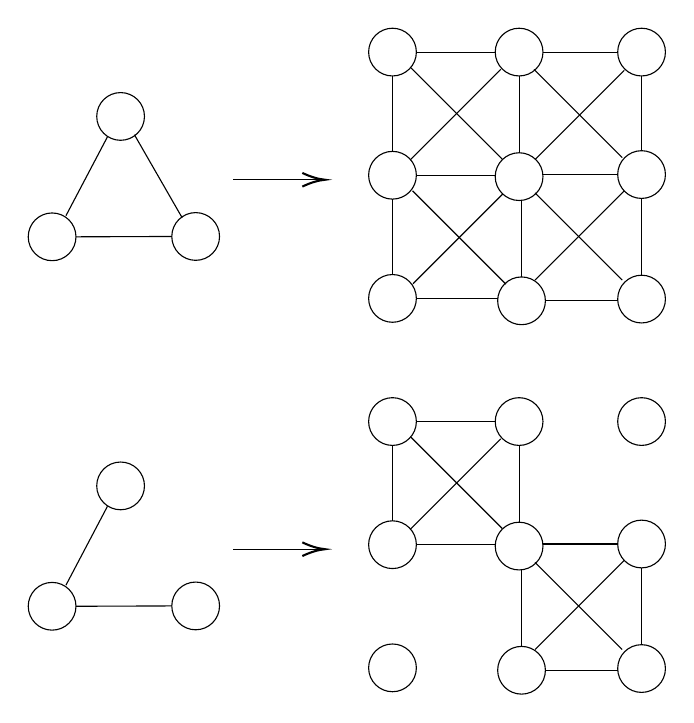
\begin{tikzpicture}[x=0.75pt,y=0.75pt,yscale=-1,xscale=1]
%uncomment if require: \path (0,388); %set diagram left start at 0, and has height of 388

%Shape: Circle [id:dp2354998254867846] 
\draw   (221,70.5) .. controls (221,64.15) and (226.15,59) .. (232.5,59) .. controls (238.85,59) and (244,64.15) .. (244,70.5) .. controls (244,76.85) and (238.85,82) .. (232.5,82) .. controls (226.15,82) and (221,76.85) .. (221,70.5) -- cycle ;
%Shape: Circle [id:dp0003468264981381086] 
\draw   (188,128.5) .. controls (188,122.15) and (193.15,117) .. (199.5,117) .. controls (205.85,117) and (211,122.15) .. (211,128.5) .. controls (211,134.85) and (205.85,140) .. (199.5,140) .. controls (193.15,140) and (188,134.85) .. (188,128.5) -- cycle ;
%Shape: Circle [id:dp4134071778258759] 
\draw   (257.17,128.33) .. controls (257.17,121.98) and (262.32,116.83) .. (268.67,116.83) .. controls (275.02,116.83) and (280.17,121.98) .. (280.17,128.33) .. controls (280.17,134.68) and (275.02,139.83) .. (268.67,139.83) .. controls (262.32,139.83) and (257.17,134.68) .. (257.17,128.33) -- cycle ;
%Straight Lines [id:da03322506525937774] 
\draw    (226.17,80.33) -- (206.17,118.33) ;
%Straight Lines [id:da10829630530082368] 
\draw    (239.17,79.33) -- (262.17,119.33) ;
%Straight Lines [id:da09584382201131803] 
\draw    (211,128.5) -- (257.17,128.33) ;
%Shape: Circle [id:dp4951446020026069] 
\draw   (352,39.5) .. controls (352,33.15) and (357.15,28) .. (363.5,28) .. controls (369.85,28) and (375,33.15) .. (375,39.5) .. controls (375,45.85) and (369.85,51) .. (363.5,51) .. controls (357.15,51) and (352,45.85) .. (352,39.5) -- cycle ;
%Shape: Circle [id:dp9466683132899918] 
\draw   (352,98.83) .. controls (352,92.48) and (357.15,87.33) .. (363.5,87.33) .. controls (369.85,87.33) and (375,92.48) .. (375,98.83) .. controls (375,105.18) and (369.85,110.33) .. (363.5,110.33) .. controls (357.15,110.33) and (352,105.18) .. (352,98.83) -- cycle ;
%Shape: Circle [id:dp5785839671866841] 
\draw   (414.17,159.33) .. controls (414.17,152.98) and (419.32,147.83) .. (425.67,147.83) .. controls (432.02,147.83) and (437.17,152.98) .. (437.17,159.33) .. controls (437.17,165.68) and (432.02,170.83) .. (425.67,170.83) .. controls (419.32,170.83) and (414.17,165.68) .. (414.17,159.33) -- cycle ;
%Shape: Circle [id:dp7410083426882006] 
\draw   (352,158.17) .. controls (352,151.82) and (357.15,146.67) .. (363.5,146.67) .. controls (369.85,146.67) and (375,151.82) .. (375,158.17) .. controls (375,164.52) and (369.85,169.67) .. (363.5,169.67) .. controls (357.15,169.67) and (352,164.52) .. (352,158.17) -- cycle ;
%Shape: Circle [id:dp8732476751204226] 
\draw   (472,158.5) .. controls (472,152.15) and (477.15,147) .. (483.5,147) .. controls (489.85,147) and (495,152.15) .. (495,158.5) .. controls (495,164.85) and (489.85,170) .. (483.5,170) .. controls (477.15,170) and (472,164.85) .. (472,158.5) -- cycle ;
%Shape: Circle [id:dp45985968503868024] 
\draw   (472,98.5) .. controls (472,92.15) and (477.15,87) .. (483.5,87) .. controls (489.85,87) and (495,92.15) .. (495,98.5) .. controls (495,104.85) and (489.85,110) .. (483.5,110) .. controls (477.15,110) and (472,104.85) .. (472,98.5) -- cycle ;
%Shape: Circle [id:dp311629952716419] 
\draw   (472,39.5) .. controls (472,33.15) and (477.15,28) .. (483.5,28) .. controls (489.85,28) and (495,33.15) .. (495,39.5) .. controls (495,45.85) and (489.85,51) .. (483.5,51) .. controls (477.15,51) and (472,45.85) .. (472,39.5) -- cycle ;
%Shape: Circle [id:dp2200025914262984] 
\draw   (413,39.5) .. controls (413,33.15) and (418.15,28) .. (424.5,28) .. controls (430.85,28) and (436,33.15) .. (436,39.5) .. controls (436,45.85) and (430.85,51) .. (424.5,51) .. controls (418.15,51) and (413,45.85) .. (413,39.5) -- cycle ;
%Shape: Circle [id:dp8283322839003597] 
\draw   (413,99.5) .. controls (413,93.15) and (418.15,88) .. (424.5,88) .. controls (430.85,88) and (436,93.15) .. (436,99.5) .. controls (436,105.85) and (430.85,111) .. (424.5,111) .. controls (418.15,111) and (413,105.85) .. (413,99.5) -- cycle ;
%Straight Lines [id:da30411841503631254] 
\draw    (363.5,51) -- (363.5,87.33) ;
%Straight Lines [id:da11066243018971855] 
\draw    (363.5,110.33) -- (363.5,146.67) ;
%Straight Lines [id:da47057554993472617] 
\draw    (375,158.17) -- (414.17,158.17) ;
%Straight Lines [id:da03822947572603663] 
\draw    (437.17,159.33) -- (472,159.33) ;
%Straight Lines [id:da5262911047621563] 
\draw    (436,98.5) -- (472,98.5) ;
%Straight Lines [id:da9258116893539396] 
\draw    (436,39.5) -- (472,39.5) ;
%Straight Lines [id:da21705787267170562] 
\draw    (375,39.5) -- (413,39.5) ;
%Straight Lines [id:da847571544559321] 
\draw    (424.5,51) -- (424.5,88) ;
%Straight Lines [id:da3839058507398059] 
\draw    (432.17,91.33) -- (475.17,48.33) ;
%Straight Lines [id:da7349542264809032] 
\draw    (373.42,151.08) -- (416.67,107.83) ;
%Straight Lines [id:da029954024979513827] 
\draw    (418.17,151.33) -- (373.17,106.33) ;
%Straight Lines [id:da7418819383595239] 
\draw    (416.42,91.08) -- (372.42,47.08) ;
%Straight Lines [id:da3388902085994645] 
\draw    (483.5,51) -- (483.5,87) ;
%Straight Lines [id:da9333917232209323] 
\draw    (483.5,110) -- (483.5,147) ;
%Straight Lines [id:da06867623129926015] 
\draw    (474.17,149.33) -- (432.17,107.33) ;
%Straight Lines [id:da2938276171928673] 
\draw    (372,91.5) -- (415.67,47.83) ;
%Straight Lines [id:da27290749951870197] 
\draw    (375,98.83) -- (413,98.83) ;
%Straight Lines [id:da502578406534109] 
\draw    (425.67,110.83) -- (425.67,147.83) ;
%Straight Lines [id:da01470667060760289] 
\draw    (432.17,149.33) -- (475.17,106.33) ;
%Straight Lines [id:da8058271357695179] 
\draw    (474.17,90.33) -- (431.67,47.83) ;
%Straight Lines [id:da5393221056920912] 
\draw    (286.67,101) -- (329,101) ;
\draw [shift={(331,101)}, rotate = 180] [color={rgb, 255:red, 0; green, 0; blue, 0 }  ][line width=0.75]    (10.93,-3.29) .. controls (6.95,-1.4) and (3.31,-0.3) .. (0,0) .. controls (3.31,0.3) and (6.95,1.4) .. (10.93,3.29)   ;
%Shape: Circle [id:dp9003325340389046] 
\draw   (221,248.5) .. controls (221,242.15) and (226.15,237) .. (232.5,237) .. controls (238.85,237) and (244,242.15) .. (244,248.5) .. controls (244,254.85) and (238.85,260) .. (232.5,260) .. controls (226.15,260) and (221,254.85) .. (221,248.5) -- cycle ;
%Shape: Circle [id:dp3392496389725759] 
\draw   (188,306.5) .. controls (188,300.15) and (193.15,295) .. (199.5,295) .. controls (205.85,295) and (211,300.15) .. (211,306.5) .. controls (211,312.85) and (205.85,318) .. (199.5,318) .. controls (193.15,318) and (188,312.85) .. (188,306.5) -- cycle ;
%Shape: Circle [id:dp980392371478102] 
\draw   (257.17,306.33) .. controls (257.17,299.98) and (262.32,294.83) .. (268.67,294.83) .. controls (275.02,294.83) and (280.17,299.98) .. (280.17,306.33) .. controls (280.17,312.68) and (275.02,317.83) .. (268.67,317.83) .. controls (262.32,317.83) and (257.17,312.68) .. (257.17,306.33) -- cycle ;
%Straight Lines [id:da7326090446149245] 
\draw    (226.17,258.33) -- (206.17,296.33) ;
%Straight Lines [id:da5243050389859094] 
\draw    (211,306.5) -- (257.17,306.33) ;
%Shape: Circle [id:dp3010486994546322] 
\draw   (352,217.5) .. controls (352,211.15) and (357.15,206) .. (363.5,206) .. controls (369.85,206) and (375,211.15) .. (375,217.5) .. controls (375,223.85) and (369.85,229) .. (363.5,229) .. controls (357.15,229) and (352,223.85) .. (352,217.5) -- cycle ;
%Shape: Circle [id:dp21234607578201947] 
\draw   (352,276.83) .. controls (352,270.48) and (357.15,265.33) .. (363.5,265.33) .. controls (369.85,265.33) and (375,270.48) .. (375,276.83) .. controls (375,283.18) and (369.85,288.33) .. (363.5,288.33) .. controls (357.15,288.33) and (352,283.18) .. (352,276.83) -- cycle ;
%Shape: Circle [id:dp4869769848436598] 
\draw   (414.17,337.33) .. controls (414.17,330.98) and (419.32,325.83) .. (425.67,325.83) .. controls (432.02,325.83) and (437.17,330.98) .. (437.17,337.33) .. controls (437.17,343.68) and (432.02,348.83) .. (425.67,348.83) .. controls (419.32,348.83) and (414.17,343.68) .. (414.17,337.33) -- cycle ;
%Shape: Circle [id:dp17917804753313038] 
\draw   (352,336.17) .. controls (352,329.82) and (357.15,324.67) .. (363.5,324.67) .. controls (369.85,324.67) and (375,329.82) .. (375,336.17) .. controls (375,342.52) and (369.85,347.67) .. (363.5,347.67) .. controls (357.15,347.67) and (352,342.52) .. (352,336.17) -- cycle ;
%Shape: Circle [id:dp2348365101098342] 
\draw   (472,336.5) .. controls (472,330.15) and (477.15,325) .. (483.5,325) .. controls (489.85,325) and (495,330.15) .. (495,336.5) .. controls (495,342.85) and (489.85,348) .. (483.5,348) .. controls (477.15,348) and (472,342.85) .. (472,336.5) -- cycle ;
%Shape: Circle [id:dp5068654492520597] 
\draw   (472,276.5) .. controls (472,270.15) and (477.15,265) .. (483.5,265) .. controls (489.85,265) and (495,270.15) .. (495,276.5) .. controls (495,282.85) and (489.85,288) .. (483.5,288) .. controls (477.15,288) and (472,282.85) .. (472,276.5) -- cycle ;
%Shape: Circle [id:dp7567362172539573] 
\draw   (472,217.5) .. controls (472,211.15) and (477.15,206) .. (483.5,206) .. controls (489.85,206) and (495,211.15) .. (495,217.5) .. controls (495,223.85) and (489.85,229) .. (483.5,229) .. controls (477.15,229) and (472,223.85) .. (472,217.5) -- cycle ;
%Shape: Circle [id:dp316640742806896] 
\draw   (413,217.5) .. controls (413,211.15) and (418.15,206) .. (424.5,206) .. controls (430.85,206) and (436,211.15) .. (436,217.5) .. controls (436,223.85) and (430.85,229) .. (424.5,229) .. controls (418.15,229) and (413,223.85) .. (413,217.5) -- cycle ;
%Shape: Circle [id:dp5619383004619796] 
\draw   (413,277.5) .. controls (413,271.15) and (418.15,266) .. (424.5,266) .. controls (430.85,266) and (436,271.15) .. (436,277.5) .. controls (436,283.85) and (430.85,289) .. (424.5,289) .. controls (418.15,289) and (413,283.85) .. (413,277.5) -- cycle ;
%Straight Lines [id:da38069948536852505] 
\draw    (363.5,229) -- (363.5,265.33) ;
%Straight Lines [id:da34936280325188496] 
\draw    (437.17,337.33) -- (472,337.33) ;
%Straight Lines [id:da49135062694874043] 
\draw    (436,276.5) -- (472,276.5) ;
%Straight Lines [id:da2779507197021105] 
\draw    (375,217.5) -- (413,217.5) ;
%Straight Lines [id:da1068062517370798] 
\draw    (424.5,229) -- (424.5,266) ;
%Straight Lines [id:da01680731608306152] 
\draw    (416.42,269.08) -- (372.42,225.08) ;
%Straight Lines [id:da6138746171180613] 
\draw    (483.5,288) -- (483.5,325) ;
%Straight Lines [id:da961665446077739] 
\draw    (474.17,327.33) -- (432.17,285.33) ;
%Straight Lines [id:da46102906626653617] 
\draw    (372,269.5) -- (415.67,225.83) ;
%Straight Lines [id:da17383285456477537] 
\draw    (375,276.83) -- (413,276.83) ;
%Straight Lines [id:da13886218938951944] 
\draw    (425.67,288.83) -- (425.67,325.83) ;
%Straight Lines [id:da5333494579056659] 
\draw    (432.17,327.33) -- (475.17,284.33) ;
%Straight Lines [id:da8834763590110171] 
\draw    (286.67,279) -- (329,279) ;
\draw [shift={(331,279)}, rotate = 180] [color={rgb, 255:red, 0; green, 0; blue, 0 }  ][line width=0.75]    (10.93,-3.29) .. controls (6.95,-1.4) and (3.31,-0.3) .. (0,0) .. controls (3.31,0.3) and (6.95,1.4) .. (10.93,3.29)   ;




\end{tikzpicture}

\textbf{\\ \\G $\rightarrow$ G'}
\begin{align*}
    G' = G\times G &=(V',E')\\
    V' &= V \times V\\
    \{(u,v), (w,x)\} \ \in E'\ \mathbf{iff}\ [\{( u,w)\} \in E\ &\mathbf{or} \ u=w] \ \mathbf{and}\ [\{( v,x)\} \in E\ \mathbf{or} \ v=x]
\end{align*}
\end{center}